\newpage
\section{Evaluation}
For the evaluation of the user experience, 14 users have been presented who test the tool freely.
After a week, test users are proposed a survey that contains questions about understandability
of information and about usability. Also, in the case of the questions so that the
Respondents can make their own contributions.
\begin{figure}[ht]
   \centering
   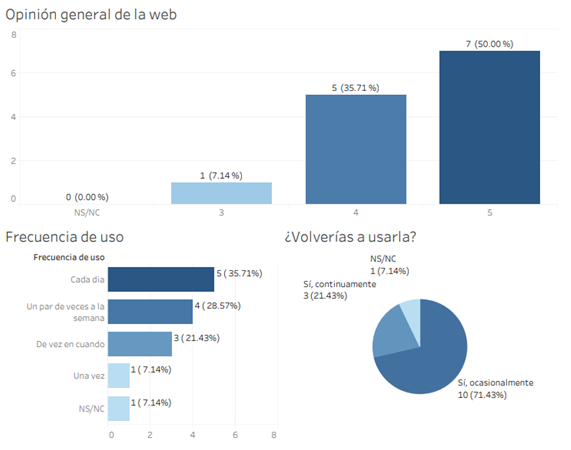
\includegraphics[width=12cm]{enqueteResults}
   \caption{Part of the user experience enquete results}
\end{figure}

Regarding the comments, most of the respondents agree that the functionality they liked the most is to see in the
map the air quality index and suggest an enlargement the number of zones.
92 \% of the respondents find the information useful and complete and 71.43 \% have answered that they also find it
understandable.
More than half of the respondents admit that they did not know the meaning of the air quality index, but after
consult the help, they have understood it.
Regarding their interests on air quality, half of them indicate that they have ever sought information about it,
only two are well informed and one of them marks the other option and specifies that it has aroused their interest after using
the application.
In addition, four of them indicate that they have discovered that they have a medical condition that affects the quality of the air thanks
to the tool.

Among the test subjects, a greater awareness of pollution has been recognized, showing more interest in the
air quality in the city and its possible effects on health
